% 解析坐标严格确定：圆 x^2+y^2=25，A=(3,4), B=(3,-4), M=(3,0)
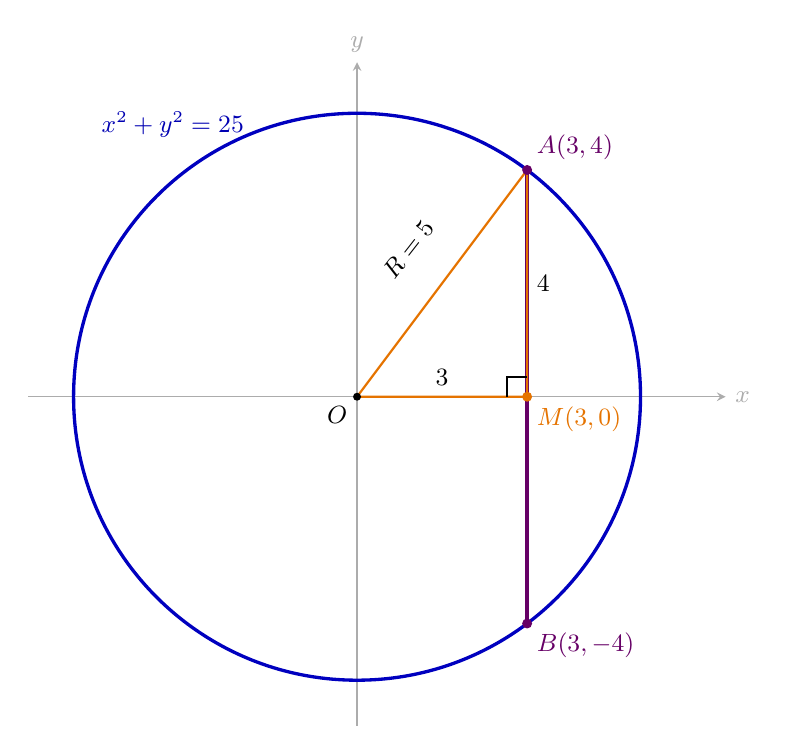
\begin{tikzpicture}[scale=.72,>=stealth,font=\small]
  \draw[->,gray!65] (-5.8,0)--(6.5,0) node[right] {$x$};
  \draw[->,gray!65] (0,-5.8)--(0,5.9) node[above] {$y$};
  \draw[very thick,blue!75!black] (0,0) circle (5);
  \draw[very thick,violet!80!black] (3,-4)--(3,4);
  \draw[thick,orange!90!black] (0,0)--(3,0)--(3,4)--cycle;
  \draw[black,thick] (2.65,0)--(2.65,.35)--(3,.35);
  \fill[black] (0,0) circle(2pt) node[below left] {$O$};
  \fill[orange!90!black] (3,0) circle(2.5pt) node[below right] {$M(3,0)$};
  \fill[violet!80!black] (3,4) circle(2.5pt) node[above right] {$A(3,4)$};
  \fill[violet!80!black] (3,-4) circle(2.5pt) node[below right] {$B(3,-4)$};
  \node[above] at (1.5,0.03) {$3$};
  \node[right] at (3,2.0) {$4$};
  \node[rotate=52] at (0.9,2.6) {$R=5$};
  \node[blue!70!black] at (-3.25,4.8) {$x^2+y^2=25$};
\end{tikzpicture}
